%O+I

\ifx\wholebook\relax\else
\input{../Common.tex}
\input{../macroes.tex}
\begin{document}
\fi

\chapter{Of Robots and Men}\label{ch:TurtleMen}\label{ch:robotMen}

\begin{chapterfigure}

\includegraphics[width=0.9\linewidth]{turtleMPica}
\end{chapterfigure}

\hidden{| caro |
caro := robot new.
"letter P"
caro west; jump: 30 ;jump: 100; north.
caro go: 100; east; go: 100; south; go: 50.
caro west; go: 100; south ; jump: 50 ; east.
caro jump: 130.
"letter I"
caro north; go: 100; south; jump: 100; east; jump: 30.
"letter C" 
caro jump: 100 ; north;  jump: 100 ; west ; go: 100; 
south; go: 100; east; go: 100; jump: 30.
"letter A"
caro north.
caro go: 100.
caro east.
caro go: 100.
caro south.
caro go: 100.
caro north.
caro go: 50.
caro west.
caro go: 100.
}

In this chapter we describe the creation of robots, and the different types of movements that robots know. We propose you some simple experiments to practice what you learned in the previous chapters. We also present how robots may change direction in an absolute manner.  


\section{Creating Robots}
In the previous chapter we mentioned that we created \emph{a} robot, not \emph{the} robot. Indeed, we can create as many robots as we want. Here is a new script \ref{scr:geminiScript} that creates two robots \ct{\caro} and \ct{daly}.

\begin{scriptwithouttitle} \label{scr:geminiScript}
| \caro daly |
\caro := Bot new.
daly := Bot new.
\caro color: Color yellow.
daly jump: 100.
\end{scriptwithouttitle}

The second line creates a robot named \caro as in \scriptref{scr:firstScript}. The third line creates a new robot that we refer to using the variable \ct{daly}. Both robots are created at the same location. In line four, we ask \caro to change its color so that we can distinguish the two robots.



 \st \index{object} is an object-oriented programming language. This means that we create objects and interact with them, or that objects can create other objects and communicate with them.  Moreover, in \st, there are special objects, called  \index{class}\emph{classes}, which are used to create objects. Sending the message \ct{new}\index{\ct{new}} to classes creates an object described by its class. Sending the message \ct{new} to the \ct{Bot} class creates a robot.

To understand what  classes are imagine that a class is a factory. A factory of tin boxes creates many boxes of the same size and shape. After being created, some boxes can be filled, others can be crushed. When one box is crushed, the other boxes are not crushed. The same thing happens with object created inside \sq. In our case, \caro did not move, but \ct{daly} did. You can think of a class as a factory able to produce unlimited supplies of objects of the same type. Once produced, each object exist
independently of the other. 

Class names always begin with an uppercase letter. That's why the
name of the robot class is \ct{Bot} with an uppercase ``B''.
\ct{Color} is also a class producing color objects but we should use a color name
to specify the color we want to obtain. For example, \ct{Color yellow} creates the color yellow.

\largecadre{A class is a factory of objects. Sending the message \ct{new} to a class creates an object of this class.  Class names always start with an uppercase letter. Here \ct{Bot} is the factory creating new robots and \ct{Color} the one for colors.

\begin{nalltt}
Bot new color: Color blue
\end{nalltt}}




\section{Drawing Line Segments}

Asking a robot to draw a line is rather simple as we already saw in the previous chapter. The message \ct{go: 100} asks a robot to move ahead 100 pixels and it leaves a trace during its move. However, even if you were an expert Chinese or Japanese caligrapher, you need to lift the brush from time to time when you drawing. For this purpose a robot knows how to jump, \ie moving forward without leaving a trace. A robot understands the message \ct{jump:}, the argument is the same as with \go, it is a distance in number of pixels. Here is a script which draws two segments. Note that we are hiding the robots from the illustration using the message \ct{beInvisible} so that you can get clearer pictures.

\begin{scriptfig}{turtleMTwoLines}{Two lines}\label{scr:twoLines}
| \caro | 
\caro := Bot new.
\caro go: 30.
\caro jump: 30.
\caro go: 30.
\end{scriptfig}

\begin{exonofig}
Experiment by changing the values in the previous script. 
\end{exonofig}

\begin{exofigwithsize}[0.5]{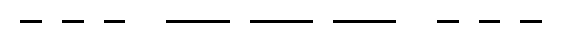
\includegraphics[width=6cm]{turtleMSosLines}}\label{exo:sosLines} 
Generate a script able to draw an SOS message using Morse code.  In
Morse, an "S" is represented by 3 short lines and an "O" is
represented by three long lines as shown by figure on the right.
\end{exofigwithsize}



\section{Changing Directions}
A robot can orient itself along the eight directions as shown by Figure~\ref{fig:roseDesVents}. These directions are like those of a map: east is pointing to the right, west to the left, north up, and south down. To make a robot pointing in a given direction just send it a message with the name of the direction.  So, to ask \caro to face south, one simply types \ct{\caro south}. 

Robots understand  the following messages: \ct{east}, \ct{north}, \ct{northEast}, \ct{northWest}, \ct{south}, \ct{southEast}, \ct{southWest} and \ct{west}. Note that in the next chapter we shall show you how to make a robot turns in a relative manner and from any angle. 

\begin{figure}
\center{\includegraphics[width=10cm]{roseDesVents}}
\caption{The default absolute directions to which a robot can point to.\label{fig:roseDesVents}}
\end{figure}


The script~\ref{scr:mappingrobot} illustrates simply the basic four directions with four different robots. In this script, we use four different robots. Each of them, except
\caro, is oriented toward a different direction before moving. Now we can use the orientation methods to make more complex drawings. As a first exercise draw  a square of 50 pixels size. Then draw another square of 250 pixels.  

\begin{scriptwithtitle}{A gaggle of robots}\label{scr:mappingrobot}
| \caro daly klee sisl |
\caro := Bot new.
\caro color: Color green.
\caro go: 100.
daly := Bot new.
daly north.
daly color: Color yellow.
daly go: 100.
klee := Bot new.
klee west.
klee color: Color red.
klee go: 100.
sisl := Bot new.
sisl south.
sisl go: 100.
\end{scriptwithtitle}


\begin{exofig}{turtleMSmallStairs}
Hopefully we are not limited to squares. One can do a wide range of geometrical figures. For example, here is a drawing of a small stairs. Define the script that reproduces it.
\end{exofig}

%\includegraphics[width=4cm]{robotMSquare}

%Try to define such a script before reading the following one: 

%\begin{scriptfigwithsize}[0.4]{}{A first square}\label{scr:firstSquare}
%| caro |
%caro := robot new.
%caro go: 100.
%caro north.
%caro go: 100.
%caro west.
%caro go: 100.
%caro south.
%caro go: 100
%\end{scriptfigwithsize}


%\begin{scriptfig}{robotMSmallStairs}{Small stairs}\label{scr:smallStairs}
%| caro |
%caro := robot new.
%caro north.
%caro go: 25.
%caro east.
%caro go: 25.
%caro north.
%caro go: 25.
%caro east.
%caro go: 25.
%caro north.
%caro go: 25.
%caro east.
%caro go: 25.
%caro north.
%caro go: 25.
%caro east.
%caro go: 25.
%caro south.
%caro go: 100.
%caro west.
%caro go: 100.
%\end{scriptfig}



\begin{exofig}{turtleMSaqqarah} \label{exo:saqqarah}
Now, we are ready to draw a schematic side view of the pyramid of
Saqqarah, built in 2500BC by Imhotep, the first known architect.
Generate a script able to draw a side view of the pyramid of
Saqqarah. This pyramid has four terrasses and its top is twice as
large than the terrasses as shown in the drawing on the right.
\end{exofig}

\begin{exofigwithtitle}{turtleMArtNouveau}{Pattern} \label{exo:artnouveau}
Draw the picture shown on the right.
\end{exofigwithtitle}

\hidden{
|caro|
caro := robot new.
caro go: 100.
caro turn: 90.
caro go: 100.
caro turn: 90.
caro go: 50.
caro turn: 90.
caro go: 50.
caro turn: 90.
caro go: 100.
caro turn: 90.
caro go: 25.
caro turn: 90.
caro go: 25.
caro turn: 90.
caro go: 50}


\section{The ABC of Drawing}\label{sec:abcDraw} 
Even though the control of the direction of the line segments is
somewhat limited, we can even start to program \caro to
write letters. The script~\ref{scr:letterA} draws an "A".

\begin{scriptfigwithsize}[0.4]{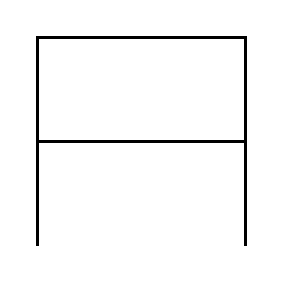
\includegraphics[width=5cm]{turtleMLetterA}}{The letter A}\label{scr:letterA}
| \caro |
\caro := Bot new.
\caro north.
\caro go: 100.
\caro east.
\caro go: 100.
\caro south.
\caro go: 100.
\caro north.
\caro go: 50.
\caro west.
\caro go: 100
\end{scriptfigwithsize}


Drawing a letter "C" is no more difficult. We can 
write a script to write "pica". 

%Here it is:

%\begin{scriptfig}[.35]{robotMBeginCaro}{The beginning of \caro}\label{scr:beginCaro}
%| caro |
%caro := robot new.
%caro west.
%caro jump: 30.
%caro go: 100.
%caro north.
%caro go: 100.
%caro east.
%caro go: 100.
%caro south.
%caro jump: 100.
%caro east.
%caro jump: 30.
%caro north.
%caro go: 100.
%caro east.
%caro go: 100.
%caro south.
%caro go: 100.
%caro north.
%caro go: 50.
%caro west.
%caro go: 100.
%\end{scriptfig}


\begin{exonofig}\label{exo:carosName} 
Draw the name of \caro. Note that as we do not want to have a line between the "C" and the "A" you should use \jump.  
\end{exonofig}

\paragraph{A Remark.}
Some purists  may think that the script~\ref{scr:letterA} could be improved. Indeed, the bottom half of  the left bar of the "A" is drawn twice since the robot is going twice
over this segment --- once going south, once going north. 
Knowing how to write the best program is a difficult question, lot of issues like the speed, the readibility of the code have to be answered and depending of the language, the methods used,..., so there is no simple answer. However, if you ask yourself such a question chose the simplest one.  Then if you have problem after because you program is too slow you can always speed it up.

\section{Controlling Robot Visibility}
We can control whether the robot should be displayed or not using the message  \ct{beInvisible} and \ct{beVisible}. \ct{beInvisible}\index{beInvisible} hides the receiver. A hidden robot acts exactly as a normal one but it just does not show where it is. Be careful attention because the method \ct{hide} already exists but it is defined by \sq and can damage the robot environment. \ct{beVisible}\index{beVisible} shows the receiving robot. A newly created robot is showing itself by default. 


\summa


\begin{table}[h]
  \centering
\begin{tabular}{| p{4cm} | p{5cm} | l |} \hline
  % after \\ : \hline or \cline{col1-col2} \cline{col3-col4} ...
  \hfil Expressions Messages & \hfil Description & \hfil Example \\[1ex] \hline
  \ct{Bot new} & Create a computer robot & \ct{pica := Bot new} \\ \hline
  \ct{| x y |} & Declare variables used in the script & \ct{| pica |} \\ \hline
  \ct{jump: anInteger}  & Ask a robot to move forward by a given number of pixels without leaving a trace & \ct{pica jump: 10} \\ \hline
  \ct{go: anInteger} & Ask a robot to move forward by a given number of pixels while leaving a trace & \ct{pica go: 10} \\ \hline
\ct{beInvisible}& Ask a robot to be invisible& pica beInvisible\\ \hline
\ct{beVisible}& Ask a robot to be visible& pica beVisilble\\ \hline
\ct{east}, \ct{north}, \ct{northEast}, \ct{northWest}, \ct{south}, \ct{southEast}, \ct{southWest} and \ct{west}& Ask a robot to point to the corresponding direction& \ct{pica north} \\ \hline
  \ct{Color }{\emph xxx} &Create a color& \ct{Color blue} \\ \hline
  \ct{color: aColor}&Ask a robot to change its color.& \ct{pica color: Color red} \\   \hline
\end{tabular}

\end{table}

\ifx\wholebook\relax\else\end{document}\fi
